% Source: https://scnajei2ds6y.feishu.cn/wiki/CMhNwcvfziNh4EkWY9DcWO9inth
% Complete source transcribed 2026-10-26; code spelling/concatenated statements follow the webpage.
\documentclass[zihao=false,fontset=windows]{ctexart}
% ctexart 不接受任意 pt 选项。正文改 {10pt}，方括号里是行距。
\usepackage{scrextend}
\changefontsizes[12pt]{10pt}

\usepackage[a4paper,left=2.35cm,right=2.35cm,top=1.7cm,bottom=1.9cm]{geometry}
\usepackage{xcolor}
\usepackage{graphicx}
\usepackage{amsmath,amssymb}
\usepackage{enumitem}
\usepackage{tabularx}
\usepackage{colortbl}
\usepackage{listings}
\usepackage{hyperref}
\usepackage[most]{tcolorbox}

\definecolor{feishuText}{RGB}{31,35,41}
\definecolor{feishuBlue}{RGB}{36,91,219}
\definecolor{feishuRed}{RGB}{216,57,49}
\definecolor{feishuGray}{RGB}{100,106,115}
\definecolor{feishuGray2}{RGB}{143,149,158}
\definecolor{feishuPinkBg}{RGB}{251,191,188}
\definecolor{quoteBar}{RGB}{51,112,255}
\definecolor{codebg}{RGB}{245,246,247}
\definecolor{codeborder}{RGB}{222,224,227}
\definecolor{inlinebg}{RGB}{242,243,245}
\definecolor{callRed}{RGB}{253,226,226}
\definecolor{callOrange}{RGB}{255,245,235}
\definecolor{callYellow}{RGB}{254,255,240}
\definecolor{callGreen}{RGB}{240,251,239}
\definecolor{callBlue}{RGB}{240,244,255}
\definecolor{callRedSoft}{RGB}{254,241,241}
\definecolor{callSun}{RGB}{255,255,204}
\definecolor{tableHead}{RGB}{242,243,245}
\definecolor{tableRule}{RGB}{222,224,227}
\definecolor{codeText}{RGB}{31,35,41}
\definecolor{codeKeyword}{RGB}{0,0,255}
\definecolor{codeComment}{RGB}{0,128,0}
\definecolor{codeString}{RGB}{163,21,21}

\setmainfont{Times New Roman}
\setCJKmainfont{Microsoft YaHei}[AutoFakeBold=2.2]
\setCJKsansfont{Microsoft YaHei}[AutoFakeBold=2.2]
\setCJKmonofont{Microsoft YaHei}[AutoFakeBold=2.2]
\setmonofont{Consolas}
\newfontfamily\emojifont{Segoe UI Emoji}

\hypersetup{
  colorlinks=true,
  urlcolor=feishuBlue,
  linkcolor=feishuBlue,
  unicode=true,
  pdftitle={MiniGPT-4(2023, KAUST)}
}

\setlength{\parindent}{0pt}
\setlength{\parskip}{0.42em}
\setlength{\fboxsep}{1.5pt}
\setlength{\emergencystretch}{3em}
\linespread{1.28}
\color{feishuText}
\arrayrulecolor{tableRule}
\urlstyle{same}

\setlist[enumerate]{label=\textcolor{feishuBlue}{\arabic*.}, leftmargin=1.7em, itemsep=0.22em, topsep=0.28em, parsep=0.08em, partopsep=0pt}
\setlist[itemize,1]{label=\textcolor{feishuBlue}{\textbullet}, leftmargin=1.35em, itemsep=0.18em, topsep=0.25em, parsep=0.06em, partopsep=0pt}
\setlist[itemize,2]{label=\textcolor{feishuBlue}{◦}, leftmargin=1.45em, itemsep=0.12em, topsep=0.15em}
\setlist[itemize,3]{label=\textcolor{feishuBlue}{\rule[0.18em]{0.38em}{0.38em}}, leftmargin=1.55em, itemsep=0.1em, topsep=0.12em}

\newcommand{\feiEmoji}[1]{{\emojifont #1}}
\newcommand{\incode}[1]{\colorbox{inlinebg}{\ttfamily\small #1}}
\newcommand{\bigmath}[1]{%
  \begin{center}\large$\displaystyle #1$\end{center}%
}

\lstset{
  language=Python,
  basicstyle=\ttfamily\footnotesize\color{codeText},
  keywordstyle=\color{codeKeyword},
  commentstyle=\color{codeComment},
  stringstyle=\color{codeString},
  showstringspaces=false,
  breaklines=true,
  columns=fullflexible,
  keepspaces=true,
  tabsize=4,
  upquote=true,
  aboveskip=2pt,
  belowskip=0pt,
  xleftmargin=0pt,
  frame=none
}

\tcbset{
  feishubase/.style 2 args={
    enhanced,
    boxrule=0pt,
    arc=8pt,
    left=10pt,
    right=10pt,
    top=7pt,
    bottom=7pt,
    before skip=6pt,
    after skip=6pt,
    colback=#1,
    colframe=#1,
    before upper={\feiEmoji{#2}\hspace{0.45em}\ignorespaces}
  }
}
\newtcolorbox{feishubox}[2]{feishubase={#1}{#2}, breakable}
\newtcolorbox{feishuboxnb}[2]{feishubase={#1}{#2}}

\newtcolorbox{feishuquote}{
  enhanced,
  breakable,
  boxrule=0pt,
  leftrule=3pt,
  arc=0pt,
  colframe=quoteBar,
  colback=white,
  left=8pt,
  right=2pt,
  top=2pt,
  bottom=2pt,
  before skip=4pt,
  after skip=4pt,
  before upper=\color{feishuGray}
}

\newtcolorbox{feishucode}{
  enhanced,
  breakable,
  colback=codebg,
  colframe=codeborder,
  boxrule=0.6pt,
  arc=6pt,
  left=6pt,
  right=6pt,
  top=5pt,
  bottom=4pt,
  before skip=6pt,
  after skip=6pt
}

\definecolor{feishuGreen}{RGB}{46,161,33}
\definecolor{callSourceGreen}{RGB}{217,245,214}
\begin{document}
{\zihao{1}\bfseries MiniGPT-4(2023, KAUST)\par}

% source-block: YwQNddEcCo3xTGxKMKDc70LunQe
\begin{feishuquote}
% source-block: doxcnMzthRnQyqgKrS0j5JWBOCc
MiniGPT-4：LLM辅助多模态(2023.04, KAUST)\par

% source-block: IrbUdxpwdo1iwJxmvl2c4l37nOc
\href{https://arxiv.org/abs/2304.10592}{MiniGPT-4: Enhancing Vision-Language Understanding with Advanced Large Language Models}\par

\end{feishuquote}

% source-block: V9UHdRq0QoQYMtxod2ycmRJGnAg
MiniGPT-4是对GPT-4的多模态能力的一次探索和尝试，其实也是和LLaVA相同的目的，都认为增强多模态模型的生成能力一定要利用LLM的知识库。因此也是采用“对齐”的思路来训练一个投影层将预训练好的LLM和视觉模型链接在一起。\par

% source-block: Hyx2dps1soxAgHxBqMPcxUiSnzb
核心点：\par

\begin{itemize}
% source-block: YWNVdRdvEoXesZxHqs8cPyZgnqQ
\item 固定vision encoder和LLM，仅训练projection对齐部分，就能获得不错的效果，并且仅用一个projection layer就能实现很强大的对齐功能\par
% source-block: TREEd5z1uoRyYPxEp2FcUvqin5g
\item 仅使用image caption进行对齐并不能获得很好的效果，而用小部分的detailed image description pairs进行further finetuning就能打破这个限制\par
% source-block: RsL4dj8fDoRPOAx43KUcc7hRnDe
\item MiniGPT-4表现出了和GPT-4类似的能力，比如生成复杂的image descriptions，从手写文本生成网页，还有GPT-4没有的能力，比如从食物照片生成详细的烹饪食谱，根据图像编写故事或诗歌，为图像中的产品编写广告等\par
\end{itemize}

% source-block: K3k0dkMvdoF6xgxvpQncZeagnvc
\par\vspace{1.15em}\noindent{\zihao{-2}\bfseries 1. 模型结构}\par\vspace{0.28em}

% source-block: Dm7JdEga4ozuKkxbr9gcTJZMnCc
\begin{center}
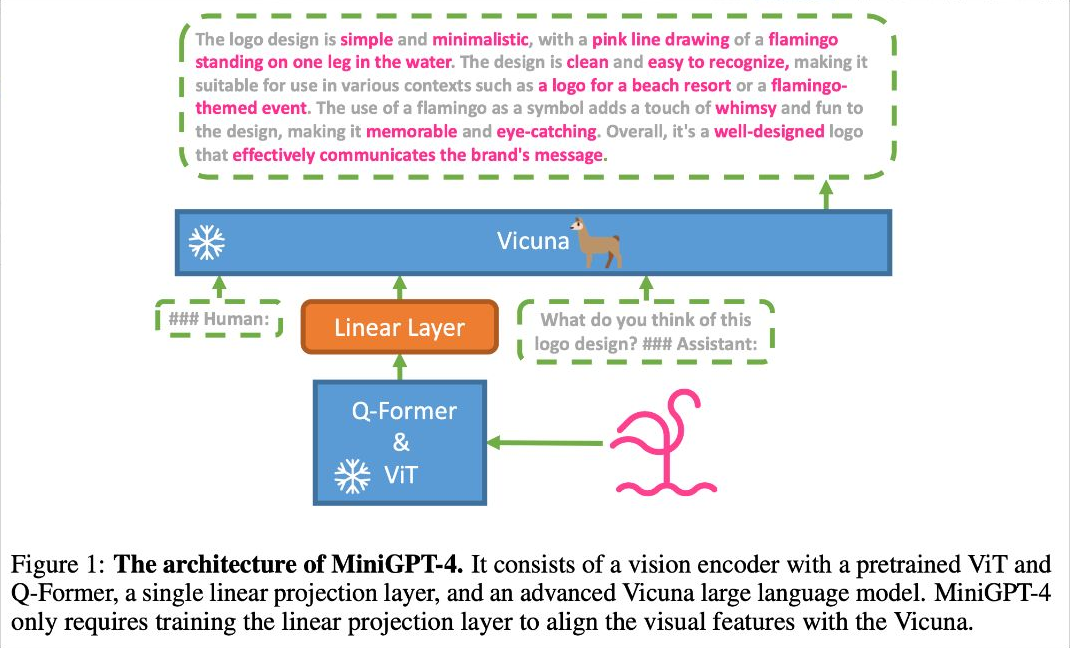
\includegraphics[width=0.98\linewidth]{images/2023-MiniGPT-4/fig-01.png}
\end{center}

\begin{itemize}
% source-block: BWKzd0DCgo3yYsxX6V5ceZJanRb
\item \colorbox{feishuPinkBg}{\textbf{视觉模块 Image Encoder}}：\par
% source-block: Pz7IddArTos7yfxUx3dc06swnOb
预训练好的\href{https://scnajei2ds6y.feishu.cn/wiki/AZiVwFmXEirI77kAVzYcOMNVnbh#NAZtdozkGoFqMQxHJgKc9rCynbe}{BLIP-2}中的视觉部分 ViT + Q-former（\feiEmoji{⚠} \textcolor{feishuGreen}{Q-former这里只有视觉的输入，没有文本的输入}）\par

% source-block: JxzPdHEQPoyRM0xvCzZcNUpUnnd
\item \colorbox{feishuPinkBg}{\textbf{对齐模块 Projection layer}}：\par
% source-block: WkeEdon9poLDBKxdVkfcBCoInxb
一个线性层linear。\par

% source-block: HOZSd1NJJoKgdZx9yMHc9tpMnSf
该线性层实际上是一个升维操作，将ViT输出的编码向量768维变为4096维（在BLIP-2中这里是2560）\par

% source-block: GbMedzovKotsGJxCuuPcSCNXn3d
\item \colorbox{feishuPinkBg}{\textbf{语言模块 LLM}}：\par
% source-block: CFfrdkrh5ox05FxHYlNcGEupnob
预训练好的Vicuna（和LLaVA用的一样）。\par

\end{itemize}

% source-block: SrC5dZlUsoOPZ0xF1fRcyGzBnzf
image encoder和LLM都不参与训练，仅训练projection的参数，降低了计算开销，训练也很高效。从上述架构可见：miniGPT4的输入是：图片和文本，输出是文本序列。\par

% source-block: BgPWdjKN7ovxvrxEaXicjKgCntg
创建projection的代码：\par

% source-block: NOBodRVj3oW1xYxGqcacgyb2ndY
\begin{feishucode}
\begin{lstlisting}
# 创建线性投影层，将经过 Q-Former 转换的图像特征映射到语言模型的嵌入空间
# img_f_dim 是图像特征的维度
# llama_model.config.hidden_size 是语言模型的隐藏状态的维度
self.llama_proj = nn.Linear(img_f_dim, self.llama_model.config.hidden_size)
\end{lstlisting}
\end{feishucode}

% source-block: Pqi8dU3vTourMtxGWdLcNP0In4f
输入图像后 MiniGPT-4 完整的处理流程：\par

% source-block: W112dm0GMoaVVWxiQXtcdQNxnnd
\begin{feishucode}
\begin{lstlisting}
def encode_img(self, image):device = image.devicewith self.maybe_autocast():
    # 使用视觉编码器对图像进行编码，再使用 LayerNorm 标准化
    image_embeds = self.ln_vision(self.visual_encoder(image)).to(device)
    # 默认使用冻结的 Q-Former
    if self.has_qformer:
    # 创建图像的注意力掩码
        image_atts = torch.ones(image_embeds.size()[:-1], dtype=torch.long).to(device)
        # 扩展查询标记以匹配图像特征的维度
        query_tokens = self.query_tokens.expand(image_embeds.shape[0], -1, -1)
        # 使用 Q-Former 模块计算查询标记和图像特征的交叉注意力，更好地对齐图像和文本
        query_output = self.Qformer.bert(query_embeds=query_tokens,encoder_hidden_states=image_embeds,encoder_attention_mask=image_atts,return_dict=True,)
        # 通过线性投影层将 Q-Former 的输出映射到语言模型的输入
        inputs_llama = self.llama_proj(query_output.last_hidden_state)
        # 创建语言模型的注意力掩码
        atts_llama = torch.ones(inputs_llama.size()[:-1], dtype=torch.long).to(image.device)
    # 返回最终输入进语言模型中的图像编码和注意力掩码
    return inputs_llama, atts_llama
\end{lstlisting}
\end{feishucode}

% source-block: LcXndBaDDoAwqkx1eqfcVqKxnHb
输入流程概括：\par

% source-block: Jkb7d0IKIoD7cDxHh7Hcp1FCn2e
输入的图片经过视觉模块进行编码得到一个图像 embedding，然后将图像 embedding 经过一个线性层与文本embedding对齐，再将原文本embedding和经过对齐后的图像embedding concat起来，输入到 LLM 中，就可以实现能够接受多模态信息的 GPT 了。\par

% source-block: A48UdhBGcoDWvkxfemScxokhn2T
\begin{feishubox}{callSourceGreen}{🙋}
% source-block: DaPddqDYKo9GIkxbfNbcTbY3ndC
在LLaVA中之用projection layer方法也尝试过了，也是比较有用的，但LLaVA还更新了LM的参数，但是MiniGPT-4没有，那性能上会有差距吗？\par

% source-block: RRBudvZmOoKPmrxWSPxceMV0nbh
\textcolor{feishuBlue}{我感觉MiniGPT-4在图像多轮对话上的能力应该是比LLaVA要差的，因为LLaVA用图片多轮对话训练过LM，肯定是有性能提升的。但是图像理解能力可能差距不大，或者MiniGPT-4还更好点。}\par

\end{feishubox}

% source-block: NOhkd7wyLoLKlrxgiiOcL5QrnFg
\par\vspace{1.15em}\noindent{\zihao{-2}\bfseries 2. 训练方法}\par\vspace{0.28em}

% source-block: O5CRdLXjzokzYUxsD7ZcdDSWnQb
MiniGPT-4 也是\textbf{两阶段}的训练方法：\textcolor{feishuRed}{\textbf{模型预训练和模型微调}}\par

\begin{itemize}
% source-block: PDVtddB9tomPfaxvehPccn8OnTe
\item Stage-1 预训练，MiniGPT-4 在大量的图像-文本对数据上进行预训练，以获得基础的视觉语言知识；\par
% source-block: E4DydnwqSoL5f1x6IbFcpwf6nfd
\item Stage-2 微调，MiniGPT-4 使用数量更少但质量更高的图像-文本数据集进行微调，以进一步提高预训练 模型的生成质量与综合表现。\par
\end{itemize}

% source-block: C7KBdhsEbo2NX5xF5c1cvXMKn6d
\begin{center}
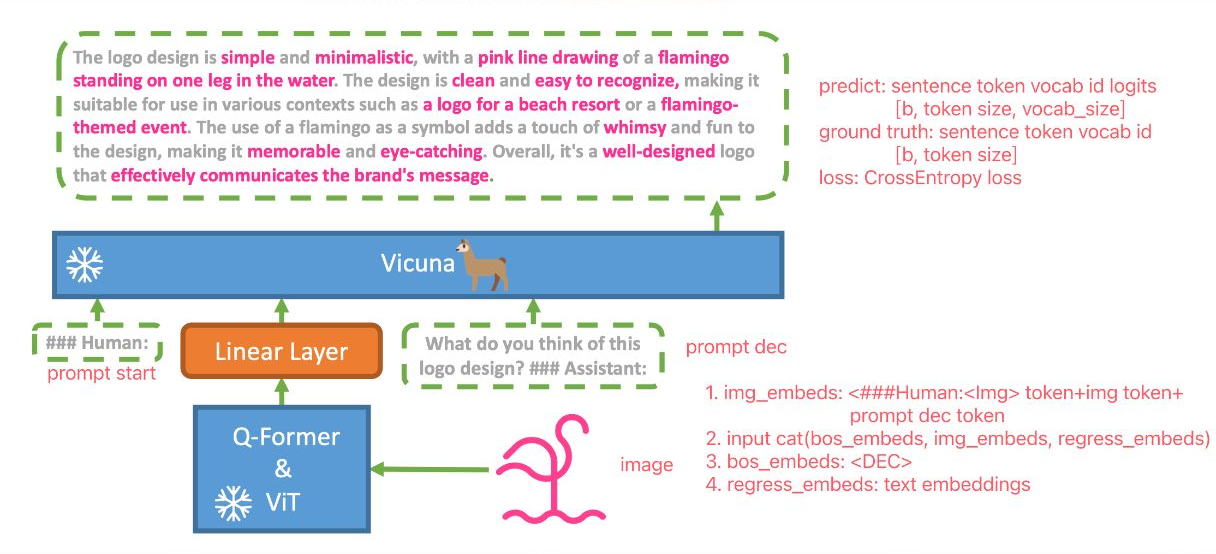
\includegraphics[width=0.98\linewidth]{images/2023-MiniGPT-4/fig-02.png}
\end{center}

% source-block: Cdrbd6s5xoHDwRxLNkDcd1hmnTh
\par\vspace{0.95em}\noindent{\zihao{3}\bfseries 2.1 Stage-1 预训练}\par\vspace{0.28em}

\begin{itemize}
% source-block: C3g7dVRvDoZORDxCNa3c3hbqnEf
\item 目标：模型需要从大量对齐的图像-文本对中获取视觉-语言知识，loss是交叉熵。\par
% source-block: SRendcXYPoamfpxkTNacR0hRn8m
\item LLM的输入（3部分组成）：\par
% source-block: DgRnd5zvgojirQxund6c4uU4nIf
句子开始标志符编码bos\_emds + 图像编码特征img\_embeds + 图像对应的描述句子编码regress\_embeds\par

% source-block: LfSqdyCelo3LqDxt4WPcDeWSnxf
\textcolor{feishuGreen}{没有上图中2个绿色部分输入（prompt start和prompt dec），只有Linear Layer的输出作为输入，加上文本tokenizer进行embedding之后，连接在一起输入给LLM}\par

\end{itemize}

\begin{itemize}
% source-block: Vu2Ydj4Q8otkKrx6DTNcOzC0nSE
\item Projection的输出可以看作是 LLM 的soft prompt，提示LLM生成相应的真实文本。\par
% source-block: CxYSd8HfXoyF89xEBRxcj4zsnfb
\item 在整个预训练过程中，预训练的\textbf{视觉编码器和LLM都保持冻结状态}，\textcolor{feishuRed}{\textbf{只有线性投影层被用来预训练}}。\par
% source-block: C5UYdH9UMoye4nxaqfgcLoIInSc
\item 使用的数据集包括 Conceptual Caption、SBU和 LAION。\par
\end{itemize}

% source-block: V7SSdLP0yojQdGxyCtIcKEyDn7d
训练了 2w 步左右，批量大小为 256，覆盖大约 500 万个图像文本对。整个过程大约需要 10 个小时才能完成，使用 4 张 A100 (80GB) GPU。\par

% source-block: C7XzdR4SwopG7zx8Cn3co8Fznjh
但是，在第一阶段预训练完成后，MiniGPT-4有一定的图文响应能力，但是生成并不流畅，会有\textbf{重复说话，句子碎片化，输出不相干}等问题(这也是多模态大模型的常见问题了)。\par

% source-block: YbT7dKxCioma4ExQhBkcbe3dnqf
输入embedding代码：\par

% source-block: HIMCdDx1yoygztxWiwvcZHWfnrf
\begin{feishucode}
\begin{lstlisting}
# img_embeds：vit+Q-former+line proj输出
img_embeds, atts_img = self.encode_img(image) 

# 对句子的开始标志编码
# embed_tokens = nn.Embedding(config.vocab_size, config.hidden_size, self.padding_idx),用于对词向量降维
bos_embeds = self.llama_model.model.embed_tokens(bos)


# text为图像的文本描述
text = [t + self.end_sym for t in samples["text_input"]]
to_regress_tokens = self.llama_tokenizer(
            text,
            return_tensors="pt",
            padding="longest",
            truncation=True,
            max_length=self.max_txt_len, #默认160,只编码句子的一部分
            add_special_tokens=False
        ).to(image.device)  # text to tokens

# 对文本tokenizer之后的词id进行编码，也传入作为embed去训练
to_regress_embeds = self.llama_model.model.embed_tokens(to_regress_tokens.input_ids) 
inputs_embeds = torch.cat([bos_embeds, img_embeds, to_regress_embeds], dim=1)
\end{lstlisting}
\end{feishucode}

% source-block: QcVldLMnpoILUAx9gOMc2zwcnZc
下面一段\href{https://qmmms.github.io/posts/MiniGPT-4/}{示例代码}，有助于更好地理解 MiniGPT-4 的 训练过程，实现了整个 MiniGPT-4 模型的前向传播过程，包括图像和文本的编码、提示处理、多 模态数据编码的连接，以及最终损失的计算。\par

% source-block: M7GZdbzu3oEUNDxMtKhcbW5Lnec
\begin{feishucode}
\begin{lstlisting}
def forward(self, samples):
    image = samples["image"]
    # 对输入图像进行编码
    img_embeds, atts_img = self.encode_img(image)
    # 生成文本指令
    instruction = samples["instruction_input"] if "instruction_input" in samples else None
    # 将指令包装到提示中
    img_embeds, atts_img = self.prompt_wrap(img_embeds, atts_img, instruction)
    # 配置 tokenizer 以正确处理文本输入
    self.llama_tokenizer.padding_side = "right"text = [t + self.end_sym for t in samples["answer"]]
    # 使用 tokenizer 对文本进行编码
    to_regress_tokens = self.llama_tokenizer(text,return_tensors="pt",padding="longest",truncation=True,max_length=self.max_txt_len,add_special_tokens=False).to(image.device)
    # 获取 batch_size
    batch_size = img_embeds.shape[0]
    # 创建开始符号的嵌入向量和注意力掩码
    bos = torch.ones([batch_size, 1],dtype=to_regress_tokens.input_ids.dtype,device=to_regress_tokens.input_ids.device) * self.llama_tokenizer.bos_token_idbos_embeds = self.embed_tokens(bos)atts_bos = atts_img[:, :1]
    # 连接图像编码、图像注意力、文本编码和文本注意力
    to_regress_embeds = self.embed_tokens(to_regress_tokens.input_ids)
    inputs_embeds, attention_mask, input_lens = self.concat_emb_input_output(img_embeds, atts_img, to_regress_embeds, to_regress_tokens.attention_mask)
    # 获得整体的输入编码和注意力掩码
    inputs_embeds = torch.cat([bos_embeds, inputs_embeds], dim=1)
    attention_mask = torch.cat([atts_bos, attention_mask], dim=1)
    # 创建部分目标序列，替换 PAD 标记为-100
    part_targets = to_regress_tokens.input_ids.masked_fill(to_regress_tokens.input_ids == self.llama_tokenizer.pad_token_id, -100)
    # 创建完整的目标序列，用于计算损失
    targets = (torch.ones([inputs_embeds.shape[0], inputs_embeds.shape[1]], dtype=torch.long).to(image.device).fill_(-100))
    for i, target in enumerate(part_targets):
        targets[i, input_lens[i] + 1:input_lens[i] + len(target) + 1] = target
    # 在自动混合精度环境下，计算语言模型的输出
    with self.maybe_autocast():
        outputs = self.llama_model(inputs_embeds=inputs_embeds,attention_mask=attention_mask,return_dict=True,labels=targets,)loss = outputs.loss
    # 返回损失作为输出
    return {"loss": loss}
\end{lstlisting}
\end{feishucode}

% source-block: VoeedpMHMokv4NxksVucRUYCnrg
\par\vspace{0.95em}\noindent{\zihao{3}\bfseries 2.2 构建微调数据集}\par\vspace{0.28em}

% source-block: SsNVdxqYYowOx6xdostc66vgnjg
为了优化效果，需要做第二阶段的对齐。为此MiniGPT-4专门构建了一个质量更高的指令数据集。\par

\begin{enumerate}
% source-block: DkEkdE8raob7yAxxdbXcm5thnWf
\item 作者从Conceptual Caption数据集随机挑选5000图片。用stage-1得到的模型基于下面的prompt生成详细的图像描述。\par
% source-block: XmRMdXghRoRsP3x9sGAcN2m5n8d
<ImageFeature>是上面提到的soft visual token\par

% source-block: Kr3MdU4pho0hSxxdZQvc0aMXnde
\begin{feishucode}
\begin{lstlisting}[language={}]
###Human: <Img><ImageFeature></Img>Describe this image in detail. Give as many details as possible. Say everything you see. ###Assistant:
\end{lstlisting}
\end{feishucode}

% source-block: RTTCdYTLyomkZrxivZscqgZenMh
如果生成的结果不到80个token，会增加额外的prompt \#\#\#Human: Continue \#\#\#Assistant:，以确保图片描述尽可能的详细。\par

% source-block: UjGpdVXpNoltcKxiKyIcMNTBnmg
\item 但是上面生成的结果里包含了噪声或者不连贯或者语法错误的内容，因此使用ChatGPT来修复这些问题。\par
% source-block: AhppdOC8yoGCNYxPeWUcgsx5nZf
给ChatGPT的prompt如下：\par

% source-block: DjekdtfsBoaJCbxwvIpckPJYnwc
\begin{feishucode}
\begin{lstlisting}[language={}]
Fix the error in the given paragraph. 
Remove any repeating sentences, meaningless characters, not English sentences, and so on. 
Remove unnecessary repetition. 
Rewrite any incomplete sentences.
Return directly the results without explanation. 
Return directly the input paragraph if it is already correct without explanation.
\end{lstlisting}
\end{feishucode}

% source-block: EAfndBf3Oo8o0bxV2sbcWZHOnud
\item 获得结果之后，再利用一些人工制定的规则进行筛选，比如包含“I’m sorry I made a mistake…”, 或者 “I apologize for that …”的回复可以删掉。\par
% source-block: JBTwdITd5oS1bcx2MNVcpx2gnAh
\item 最终得到了3500条高质量的数据，用于第二阶段的训练。\par
\end{enumerate}

% source-block: Xd2ZdtBgsomjR1xz0URclLrjn2d
\par\vspace{0.95em}\noindent{\zihao{3}\bfseries 2.3 Stage-2 微调}\par\vspace{0.28em}

% source-block: VB5CdHTMdoCHn4xb3edcCmEBnMg
在stage-2微调中，模型在上面生成的高质量图像-文本数据集上进行微调，仍然只训练Linear Layer，也是优化Generation Loss。\par

% source-block: RtYkdGbjkopeG8x5rEUcu1Mwndd
\feiEmoji{⚠} prompt的损失不算入训练中\par

% source-block: HLhXdatKroUZrYxjKhvcjnugnFb
第二阶段由于数据非常少，使用单个A100只要7分钟就训练完了。\par

% source-block: GLS6deRxGoj8ohx4savcS1lFnWe
\par\vspace{0.95em}\noindent{\zihao{3}\bfseries 2.4 Ablation}\par\vspace{0.28em}

% source-block: Chi2diNMgo5zZ2xdsOCcTDo5nSg
作者设计了三个实验，研究除了fine-tune新加的Linear layer，fine-tune其他的模块有用吗？\par

\begin{enumerate}
% source-block: W2N8dxxFMoYJQaxRXqfc5QEAnmf
\item 移除Q-former，直接用Projector map ViT的特征到Vicuna\par
% source-block: FdKhdhX65o9MpfxCRClcF0iDnnf
\item 用三层MLP，而不是一层\par
% source-block: VIq6dX3XUoyi1nxOVZTcnKIXn1d
\item Fine-tune Projector的同时也fine-tune Q-former\par
\end{enumerate}

% source-block: PAAxdGyuTo27u4x8acaclDpyn5e
结果如下：\par

% source-block: MNBLddQZloUe6ZxOKX0cACQynde
\begin{center}
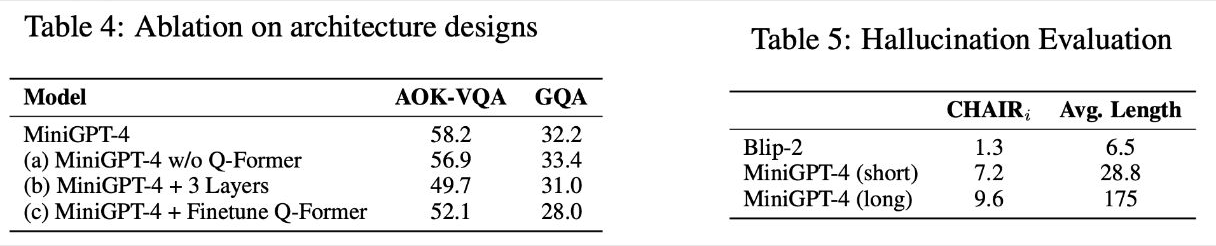
\includegraphics[width=0.98\linewidth]{images/2023-MiniGPT-4/fig-03.png}
\end{center}

% source-block: Tlt1dgCoZoTPPWx7Mb3cR6sTn5c
这个结果说明：\par

\begin{enumerate}
% source-block: XeyzduGMqoMSe5xL0I3cOHe4nze
\item 复杂的Q-former结构对alignment帮助不一定大，一层MLP Projector足矣；\par
% source-block: VyBsdliejonnpzxlUu7cjxP6nKg
\item 深层MLP映射不一定有用；\par
% source-block: FmsmdZf5qom9wfxgbDtcwlEBnCc
\item 原本Align过的Q-former如果在小的数据集上fine-tune，效果甚至可能适得其反。\par
\end{enumerate}

% source-block: KqihdAXpHoPgjnxTC2gcaCZrn8f
\par\vspace{1.15em}\noindent{\zihao{-2}\bfseries 3. 总结}\par\vspace{0.28em}

% source-block: GKiZd5DDIoPGSyxwuUKcCnsqnrh
其实MiniGPT-4没有特别大的创新，但是做了非常多实验，总结了非常多的经验，他的Ablation其实说明了很大的两点内容：\par

\begin{enumerate}
% source-block: ZKtpdf5C0oGLazxQfezcUz8dnpg
\item \textcolor{feishuRed}{高质量数据非常关键，质量 > 数量}\par
% source-block: KDvbd8XqroqDWNxay1KcAKwGnR3
\item \textcolor{feishuRed}{模态对齐模块不一定要复杂，数据才是关键}\par
\end{enumerate}

\end{document}
